% Section 2 - Docker
% Roberto Masocco <roberto.masocco@uniroma2.it>
% May 1, 2022

% ### Docker ###
\section{Docker}
\graphicspath{{figs/section2/}}

% --- Docker Engine ---
\begin{frame}{Docker Engine}
\begin{columns}
  \column{.5\textwidth}
  \textbg{Docker} is the currently de-facto standard for building, managing and distributing \textbg{multiplatform} containers.\\
  It is an engine (i.e. a collection of \textbg{daemons}) that automates the management of the kernel subsystems in order to set up, store and run containers.

  \column{.5\textwidth}
  \begin{figure}
    \centering
    \label{fig:docker}
    
\includegraphics[scale=.2]{docker.png}
    \caption{Docker logo}
  \end{figure}
\end{columns}
\end{frame}
\begin{frame}{Docker Engine}
\begin{figure}
  \centering
  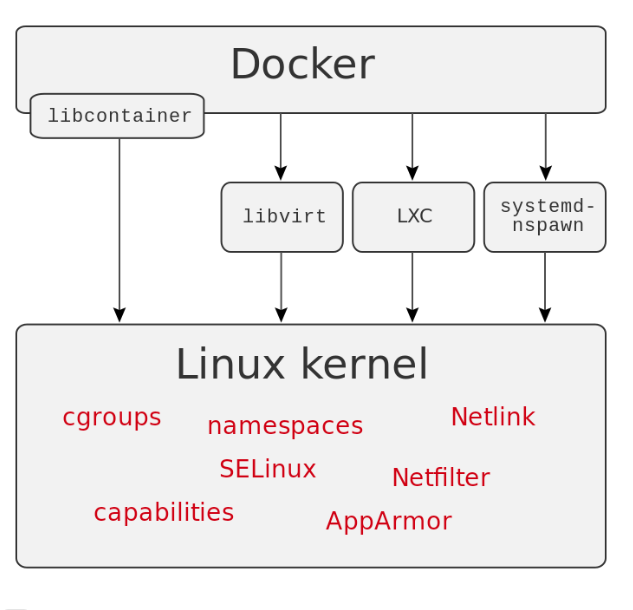
\includegraphics[scale=.3]{dockerScheme.png}
  \label{fig:dockerscheme}
  \caption{Docker Engine scheme}
\end{figure}
\end{frame}

% --- Containers in Robotics ---
\begin{frame}{Containers in Robotics}
Containers can be of help in some classic scenarios:
\begin{itemize}
  \item \textbg{deploying} applications or whole control architectures, solving issues like \textbg{dependencies} and \textbg{configurations};
  \item configuring and distributing \textbg{development environments};
  \item expanding the capabilities of \textbg{(partially) closed-source} hardware solutions (e.g. Nvidia Jetson...);
  \item working with \textbg{multiple architectures} at the same time: Docker fully supports \href{https://www.qemu.org/}{\color{blue}\textbf{\underline{QEMU}}} to build and run containers.
\end{itemize}
\end{frame}

% --- Building a Docker Container ---
\begin{frame}{Building a Docker Container}
\begin{enumerate}
  \item A \textbg{Dockerfile} specifies a set of rules to build an \textbg{image}, just like a script.
  \item \textbg{Images} are the binary archives from which a \textbg{container} can be started: they can be stored, pulled or simply built locally.
  \item A \textbg{container} can be built from an image and then started, stopped and managed by the Docker daemon.
\end{enumerate}
Images are built \textbg{incrementally}: each Dockerfile directive defines a new \textbg{layer}, and the Docker engine stores the differences between each build step thanks to filesystem capabilities: this allows to efficiently \textbg{cache build stages}.
\end{frame}

% --- Dockerfiles ---
\begin{frame}[fragile]{Dockerfiles}
\begin{columns}\column{.9\textwidth}
\begin{lstlisting}[language=Dockerfile, caption=Minimal example of a Dockerfile running an Ubuntu image in a container]
ARG VERSION=20.04
FROM ubuntu:$VERSION # Note the tag!

ENV DEBIAN_FRONTEND=noninteractive

RUN apt-get update && \
    apt-get install -y --no-install-recommends \
    build-essential \
    git && \
    rm -rf /tmp/*

ENV DEBIAN_FRONTEND=dialog
LABEL maintainer.name="Roberto Masocco"
CMD ["bash"]
\end{lstlisting}
\end{columns}
\end{frame}
\begin{frame}{Dockerfile commands}
Just to name a few (see the \href{https://docs.docker.com/engine/reference/builder/}{\color{blue}\underline{Dockerfile reference}} for more):
\begin{itemize}
  \item \texttt{FROM repository/image:tag}\\Specifies a base image to pull.
  \item \texttt{RUN command}\\Runs the following command in a new shell inside the container.
  \item \texttt{COPY source target}\\Copies a file into the container.
  \item \texttt{ENV variable=value}\\Sets an environment variable inside the container.
  \item \texttt{ARG name=value}\\Declares a build argument.
  \item \texttt{CMD ["command", "arg1", ...]}\\Specifies the command to run when the container is started.
\end{itemize}
\end{frame}

% --- Docker Commands ---
\begin{frame}{Docker Commands}
Again, just a few (each with a gazillion of options):
\begin{itemize}
  \item \texttt{docker build}\\Builds a new image from a Dockerfile.
  \item \texttt{docker run}\\Builds and starts a container.
  \item \texttt{docker ps}\\Lists active containers.
  \item \texttt{docker exec}\\Runs a command inside a container (e.g. a shell).
  \item \texttt{docker start}\\Starts a container.
\end{itemize}
\end{frame}
\begin{frame}{Docker Commands}
\begin{itemize}
  \item \texttt{docker stop}\\Stops a container.
  \item \texttt{docker images}\\Lists available images.
  \item \texttt{docker rm}\\Removes a container.
  \item \texttt{docker rmi}\\Removes an image.
\end{itemize}
Active containers are usually referenced by their \textbg{ID}.
\end{frame}
